%%%%%%%%%%%%%%%%%%%%%%%%%%%%%%%%%%%%%%%%%%%%%%%%%%%%%%%%%%%%%%%%%%%%%%%%%%%%%%%%%%%%%%%%%%%%%%%%%
\chapter{Le $\lambda$-calcul et la réduction}

\section{Définition, champ lexical et syntaxique}
Le $\lambda$-calcul est un système formel très rudimentaire. Il n'utilise que  
peu de moyens : le symbole $\lambda$, des variables et des parenthèses. Il n'a
qu'une seule règle de calcul, la $\beta$-réduction, qui modélise le passage d'un
argument à une fonction.

\begin{definition}
Un $\lambda $-terme est défini par induction de la manière suivante:
\begin{itemize}
  \item Une  variable $x$ est un $\lambda$-terme.
  \item Si $t$ est un $\lambda$-terme, l'abstraction $\lambda x.t$ est un $\lambda$-terme.
  \item Si $t_1$ et $t_2$ sont des $\lambda$-termes, l'application $(t_1 \ t_2)$ est un $\lambda$-terme.
\end{itemize}
\end{definition}

Voici le champ lexical des $\lambda $-termes:

\vspace{0.2cm}
token = \begin{tabular}{lll}
| & $\lambda$  & 	{ \verb+LAMBDA+ } \\
| & '.' &  { \verb+POINT+ } \\
| & $[ a-z ] [ a-z\  0-9 ]$ * & { \verb+VARIABLE+ } \\
| & '('	 &	{ \verb+PARLEFT+ } \\
| & ')'	 &	{ \verb+PARRIGHT+ }
\end{tabular}
\vspace{0.4cm}

Voici la grammaire des $\lambda $-termes, en utilisant les terminaux définis
avant :

\vspace{0.2cm}
\begin{tabular}{lll}
\textit{terme} ::= & | & \verb+VARIABLE+  \\
& | & \verb+PARLEFT+ \ \textit{terme} \ \textit{terme} \ \verb+PARRIGHT+ \\
& |& \verb+LAMBDA+ \ \verb+VARIABLE+ \  . \ \textit{terme}
\end{tabular}
\vspace{0.2cm}

Nous utiliserons ocamllex et menhir, qui est la version moderne de ocamlyacc, pour l'analyse lexical et syntaxique des termes
du $\lambda $-calcul.

\subsection{Analyse lexicale avec ocamllex}
Nous d\'{e}finissons ici le champ lexical des diff\'{e}rents \textit{tokens}  (\textit{l\'{e}x\`{e}mes}) du
$\lambda$-calcul.


\begin{Verbatim}
(* file: lambdalexical.mll *)
{
open Lambdagrammar (* Assumes the parser file is "lambdagrammar.mly" *)
}
let texte = ['a'-'z'] ['a'-'z' '0'-'9']*
rule token = parse
| "lambda"	{ LAMBDA }
| '.' { POINT }
| texte as varia	{ VARIABLE (varia) }
| '('		{ PARLEFT }
| ')'		{ PARRIGHT }
| _			{ token lexbuf }
| eof		{ raise End_of_file }
\end{Verbatim}

La compilation de ce fichier \verb+.mll+ va générer une fonction dont le nom
est celui de la règle (ici \verb+token+).
Cette fonction prend comme argument le type \verb+lexbuf+ et rend le type \verb+token+. 

\verb+lexbuf+  est un type de données abstrait défini dans le module Lexing 
qui permet de mémoriser la chaîne ou le fichier en cours d'analyse.
\begin{Verbatim}
val token :  Lexing.lexbuf  -> token 
\end{Verbatim}

\subsection{Analyse syntaxique avec menhir}
Nous d\'{e}finissons ici la grammaire du $\lambda$-calcul.
Nous retrouvons les constructeurs du type ML associ\'{e}s \`{a} chacune des r\`{e}gles de la grammaire.
Ces constructeurs seront préenté dans la section qui suit.


\begin{Verbatim}
/* file: lambdagrammar.mly */
%{
open Terme
%}

%token <string> VARIABLE
%token LAMBDA PARLEFT PARRIGHT POINT
%token NEWLINE

%start exp
%type <Terme.terme> exp

%% /* Grammar rules and actions follow */
exp:      VARIABLE	{ Var($1) }
| PARLEFT exp exp PARRIGHT		{ App($2, $3)}
| LAMBDA VARIABLE POINT exp		{ Lam($2, $4) }
;
%%
\end{Verbatim}



Plus exactement, nous avons modifié cette grammaire \textit{naïve} pour la
rendre non ambiguë et assurer l'associativité à gauche des
$\lambda$-applications.
En effet: 
$$ M N O P = (((M N) O) P) $$
\begin{Verbatim}
%% 
line:  exp NEWLINE { $1 }
;

exp: LAMBDA VARIABLE POINT exp		{ Lam($2, $4) }
		 | app {$1}
;

app:  atome {$1}
		 | app atome { App($1, $2) }
;

atome: PARLEFT exp PARRIGHT {$2}
       | VARIABLE {Var($1)}
;		
%%
\end{Verbatim}
Nous obtenons ainsi:
\begin{Verbatim}
$ ./lambda.out
>> m n o p
App(App(App(Var "m" ,Var "n" ),Var "o" ),Var "p" )

>> lambda f . (lambda x . f(x x)) (lambda x. f(x x))
Lam("f",App(Lam("x",App(Var "f" ,App(Var "x" ,Var "x" ))),
				Lam("x",App(Var "f" ,App(Var "x" ,Var "x" )))))
\end{Verbatim}



La compilation de ce fichier \verb+.mly+ va générer une fonction dont le nom
est celui de l'axiome de notre grammaire (ici \verb+exp+). Cette fonction prend deux arguments: la fonction de l'analyseur lexical qui génère les tokens et l'input. Elle rend le type
des expressions utilisées commes actions dans la grammaire.
\begin{Verbatim}
val exp :   (Lexing.lexbuf  -> token) -> Lexing.lexbuf -> Terme.terme
\end{Verbatim}

 Si le langage analysé n'est pas reconnu par la grammaire, l'exception \verb+Parse_error+ est levée.
 \subsection{Implémentation du parsing en mode \textit{récursif descendant}}
 
 Si nous voulons nous passer d'un outil tel que ocamlyacc ou menhir, nous pouvons très facilement implémenter un parser
 de manière récursive en partant depuis la racine (l'axiome des règles de notre grammaire) et en appelant de manière récursive les
 régles suivantes en fonction du caractère lu.
 
 On modifiera légèrement la grammaire comme ci-dessous pour faciliter le travail.
 
 
\vspace{0.5cm}
\begin{tabular}{lll}
\textit{exprule} & $::=$ & | \verb+VARIABLE+  \\
					  &	    & | \verb+PARLEFT+ \  \textit{parrule} \\
					  & 		 & | \verb+NEWLINE+ \\
\textit{parrule} & $::=$ & | \verb+LAMBDA+ \ \textit{lambdarule}  \\
					  &       & | \textit{apprule} \\ 
\textit{lambdarule} & $::=$ & \verb+VARIABLE+  \verb+POINT+  \textit{exprule}  \verb+PARRIGHT+ \\
\textit{apprule} & $::=$    &  \textit{exprule} \textit{exprule}  \verb+PARRIGHT+ \\
\end{tabular}
\vspace{0.5cm}

Cela imposera cependant la saisie systématique des $\lambda$-termes avec des parenthèses autour des abstractions et des applications.
De même, nous n'aurons plus la facilité syntaxique de l'associativité à gauche des applications et de l'associativité à droite
du corps des abstractions.
Je ne sais pas si une telle grammaire peut être conçue pour une analyse en mode
récursif descendant.
Je pense que non (après m'être un peu cassé les cheveux là-dessus... ). 

Voici le code associé.
\begin{Verbatim}
exception Fin
exception Erreur of string
	
let _ =
	let lexbuf = Lexing.from_channel stdin in
				
	let rec exprule courant =
		match courant with
		| VARIABLE(x) -> Var(x)
		| PARLEFT -> parrule (lexana lexbuf)
		| NEWLINE -> raise Fin
		| _ ->  raise (Erreur "exprule")
		
		and parrule courant =
			  match courant with
				| LAMBDA -> lambdarule courant
				| _ -> apprule courant
		 
		and apprule courant =
				let op1 = exprule courant in
			   let op2 = exprule (lexana lexbuf) in
				let suivant = lexana lexbuf in (* consume PARRIGHT*)
				match suivant with 
					| PARRIGHT ->  App(op1, op2) 
					| _ -> raise (Erreur "apprule")
		 
		and lambdarule courant =
			  let var = lexana lexbuf in 
				let _ = lexana lexbuf in  (* consume POINT *)
				let corps = exprule(lexana lexbuf) in
				let _ =  lexana lexbuf (* consume PARRIGHT *) in
				match var with 
					| VARIABLE(x) -> Lam(x, corps)
					| _ -> raise (Erreur "lambdarule")
			
		in (betaNormalPrint (exprule (lexana lexbuf)); flush stdout)
\end{Verbatim}

\section{Représentation en \textsc{Ocaml}}

\begin{Verbatim}
type terme =
| Var of string
| App of terme * terme
| Lam of variable * terme
\end{Verbatim}


Un terme du $\lambda $-calcul est donc un type ML compos\'{e}, avec les constructeurs $Var$, $App$ et $Lam$.

Par exemple, le terme $ \lambda x.(x y) z $ est represent\'{e} par la structure:



\verb+App ((Lam ("x", (App ((Var "x"), (Var "y"))))), (Var "z"))+


C'est un peu verbeux.
Voici cependant sa représentation sous la forme d'un arbre syntaxique. Le symbole @ repr\'{e}sente ici l'application.
\begin{center}
\begin{tikzpicture}[level distance=1.5cm,
level 1/.style={sibling distance=3cm},
level 2/.style={sibling distance=1.5cm}, scale=0.7]
\node{@}
child { node {$\lambda $}
		child { node {x} }
		child { node {@}
				child { node {x} }
				child { node {y} }
			  }
	  }
child { node {z} };
\end{tikzpicture}
\end{center}

Pour dessiner cet arbre, nous utilisons le tr\`{e}s bon package \textsc{Tikz} qui permet facilement de repr\'{e}senter
les arbres avec une syntaxe très simple.
\begin{Verbatim}
\node{@}
child { node {$\lambda $}
		child { node {x} }
		child { node {@}
				child { node {x} }
				child { node {y} }
			  }
	  }
child { node {z} };
\end{Verbatim}

On impl\'{e}mente deux fonctions \textsc{Ocaml}
qui permettent  d'afficher une expression de type $\lambda $-terme en code \LaTeX\ ou en code \textsc{Tikz}.



La fonction \verb+varLibres+ retourne les variables libres (ie. non li\'{e}es) d'un $\lambda $-terme.
\begin{Verbatim}
let rec varLibres lambdaTerm =
	match lambdaTerm with
	| Var x -> [ x ]
	| App (n, m) -> union (varLibres n) (varLibres m)
	| Lam (x, m) -> remove x (varLibres m)
\end{Verbatim}


Par exemple: $(\lambda x.yxw)(\lambda u.uv) \longmapsto  y,w,v $

\begin{Verbatim}
let exemple = App (Lam ("x", App (Var("y"), App (Var("x"),Var("w")))),
Lam ("u", App (Var ("u"), Var ("v")))) ;;
varLibres exemple ;;
- : variable list = ["y"; "w"; "v"]
\end{Verbatim}


\begin{definition}
Un redex ou radical est un terme de la forme $(\lambda x.M)N$
\end{definition}
On a déjà distingué deux formes possible sur les $\lambda$-termes : les \textit{abstractions} $\lambda x.M$ et les
\textit{applications} $(M N)$. Un \textit{redex} qui est de la forme $(\lambda x.M)N$ est la
rencontre d'une abstraction et d'une application. Voici son implémentation.


\vspace{0.5cm}
\begin{center}
\begin{tabular}{c | c} \hline
ML & SCHEME \\ \hline
\texttt{(function x -> M) N} &  \texttt{((lambda (x) M) N)} \\ 
\texttt{let x = N in M} & \texttt{(let ((x N)) M)} \\ 
\texttt{M where x = N} &  \\ 
\end{tabular}
\end{center}
La dernière syntaxe \texttt{M where x = N} a disparu en \textsc{Ocaml}. C'est dommage car elle est très élégante.
Nous essayerons de la reprendre pour notre interprète maison \textsc{MiniML}.

\begin{definition}
La $\beta $-r\'{e}duction est une op\'{e}ration de substitution. Elle consiste \`{a} substituer dans le redex
$(\lambda x.M) N$ les occurrences libres de x dans M par l'argument N.
On la formalise par la notation suivante:
$$
((\lambda x.M) N) \rightarrow _\beta M[x \leftarrow N]
$$
\end{definition}



Nous pouvons la décrire par les quatre règles d'inférence ci-dessous:
$$
\mathbf{(redex)} : \frac{}{((\lambda x.M)N) \rightarrow M[x \leftarrow N]} \\
$$
$$
\mathbf{(abstraction)} : \frac{M \rightarrow M_1}{ \lambda x.M \rightarrow (\lambda x.M_1)}
\quad \mathbf{(1)} : \frac{M \rightarrow M_1}{(M N) \rightarrow (M_1 N)}
\quad \mathbf{(2)} : \frac{N \rightarrow N_1}{(M N) \rightarrow (M N_1)}
$$

\vspace{0.5cm}
Pour l'implémentation, nous nous sommes appuyés sur le code de l'excellent livre \textit{Programmer avec Scheme} 
de Jacques Chazarain \cite{plisp}.  
Nous avons adapté son code \textsc{Scheme} en \textsc{Ocaml}. En comparant les deux versions, on s'aperçoit finalement
que la version \textsc{Ocaml}, même si un peu plus concise que la version \textsc{Scheme} grâce  l'utilisation du \textit{pattern matching},
reste très proche de l'original \textsc{Scheme}.

\vspace{0.5cm}
La fonction \texttt{substituer} permet de substituer la variable \texttt{var} par le terme \texttt{terme} dans l'expression \texttt{exp}.

\begin{Verbatim}
let rec substituer exp var terme =
	match exp with
	| Var x -> if x = var then terme else exp
	| App (n, m) -> App ((substituer n var terme), (substituer m var terme))
	| Lam (x, m) -> (* pas d'occurence libre on en fait rien *)
			if not (mem var (varLibres exp))
			then exp
			else (* si capture on renome *)
			if mem x (varLibres terme)
			then
				(let newV = renomme x (varLibres terme) in
					let newCorps = substituer m x (Var newV)
					in Lam (newV, (substituer newCorps var terme)))
			else  Lam (x, (substituer m var terme))
\end{Verbatim}

Avant de substituer une variable par une autre, nous devons nous assurer qu'il n'y aura pas de phénomène de capture, ie.
nous assurer qu'une variable libre ne deviendra pas liée, après substitution.
Dans l'exemple suivant, la variable x qui était libre dans $ (z x) $ se retrouve capturée par la lambda.
$$ \lambda x. (x y)[y \gets (z x)] = \lambda x.(x (z x)) $$
Pour éviter cela, il faut avant substitution opérer un renommage de la variable liée:
$$ \lambda x_1. (x_1 y)[y \gets (z x)] = \lambda x_1.(x_1 (z x)) $$
Ce renommage est appelé $\alpha$-conversion. On dit que deux termes $M$ et $N$ sont équivalents modulo $\alpha$.
On écrira $M=_\alpha N$

\begin{Verbatim}
(** renommer var *)
let renomme var listeVar =
	let rec renommeAux j =
		let varj = var ^ (string_of_int j)
		in if mem varj listeVar then renommeAux (j + 1) else varj
	in renommeAux 0
\end{Verbatim}

La fonction \texttt{reduc1Normale}  r\'{e}duit le terme en appliquant la strat\'{e}gie de r\'{e}duction normale, c'est-\`{a}-dire
en commencant la r\'{e}duction par le redex ext\`{e}rieur, plus pr\'{e}cis\'{e}ment le plus \`{a} gauche des ext\`{e}rieurs.



\begin{Verbatim}
let rec reduc1Normale terme =
   match terme with
   | Var x -> raise IRREDUCTIBLE 
   | Lam (x, m) -> Lam (x, (reduc1Normale m))
   | App (n, m) ->
	 if estRedex terme
		then betaReducRedex terme
		else
			try App ((reduc1Normale n), m)
			with IRREDUCTIBLE   -> App (n, (reduc1Normale m)) 
\end{Verbatim}

Enfin, nous avons une fonction \verb+fullReduc+ qui permet d'itérer l'opération de
$\beta$-réduction jusqu'à trouver la forme normale, ou boucler s'il n'y a pas de forme formale.
On lui impose donc maximum 1000 réductions. 
Elle prend en argument la méthode (ie. la stratégie de réduction) à  utiliser. 

\begin{Verbatim}
let rec fullReduc terme methode  =
  let rec loop terme  iter =
	try
	 let newterme = methode terme in
		if (newterme = terme || iter = 0) then newterme
		else loop newterme (iter - 1)
	with IRREDUCTIBLE -> terme	
  in loop terme 1000
	
let betaNormal t = fullReduc t reduc1Normale
\end{Verbatim}

\begin{theoreme}
La réduction normale appliquée à un terme normalisable aboutit toujours à la forme irréductible du terme.
\end{theoreme}

Nous avons en plus le théorème suivant (plus précisément son corollaire) qui nous assure que toutes les réductions d'un $\lambda$-terme (qui terminent) aboutissent au m\^{e}me
terme irréductible.



\begin{theoreme}
Théorème de Church-Rosser : la $\beta $-réduction est confluente.
\end{theoreme}
\begin{tikzpicture}
	\draw [-latex] (1,1) node[above]{$M$} --node{$*$}   (0,0) node[left]{$M_1$} ;
	\draw [-latex] (1,1) --node{$*$}  (2,0) node[right]{$M_2$};
	\draw [-latex, dotted] (0,0) --node{$*$}  (1,-1) node[below] {$M'$};
	\draw [-latex, dotted] (2,0) --node{$*$}  (1,-1) ; 
	\node [text width = 9cm] at(8,0)  {si $M \overset{*}{\longrightarrow_{\beta}} M_1$ et $M \overset{*}{\longrightarrow_{\beta}}  M_2$ alors 
	$\exists\, M'$ tel que  $M_1 \overset{*}{\longrightarrow_{\beta}}  M'$ et $M_2 \overset{*}{\longrightarrow_{\beta}}  M'$} ;
\end{tikzpicture}

\begin{theoreme}
	Corollaire du théorème de Church-Rosser \\
	Si $M$ est normalisable, il existe un unique terme normal, noté $\overline{M}$ tel 
	que $M \overset{*}{\longrightarrow_{\beta}} \overline{M}$
\end{theoreme}
Un corollaire ne devrait pas nécessiter de preuve car supposée évidente. La voici cependant:

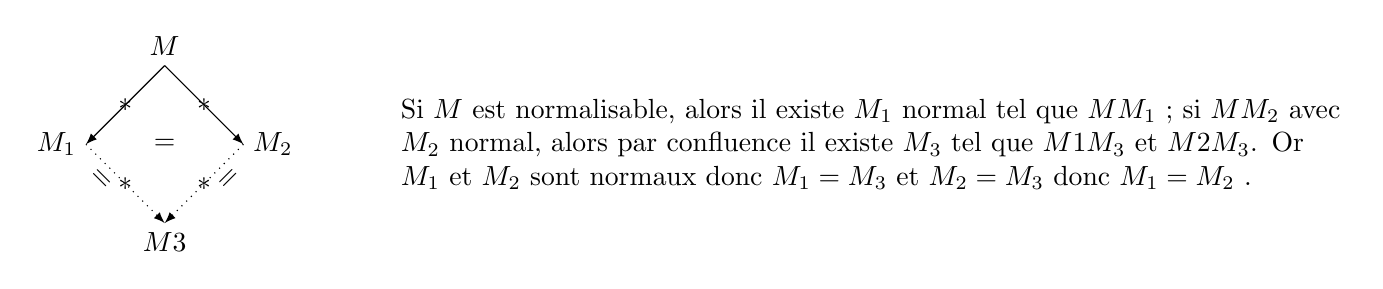
\begin{tikzpicture}
	\draw [-latex] (1,1) node[above]{$M$} --node{$*$}   (0,0) node[left]{$M_1$} ;
	\draw [-latex] (1,1) --node{$*$}  (2,0) node[right]{$M_2$};
	\draw [-latex, dotted] (0,0) --node{$*$} node[below left, sloped, midway]{$=$} (1,-1) node[below] {$M3$};
	\node at(1,0) {$=$} ; 
	\draw [-latex, dotted] (2,0) --node{$*$} node[below right, sloped, midway]{$=$} (1,-1) ; 
	\node [text width = 12cm] at(10,0)	{ Si $M$ est normalisable, alors il existe $M_1$ normal
	tel que $M \trans M_1$ ; si $M \trans M_2$ avec
	$M_2$ normal, alors par confluence il existe $M_3$ tel que $M1 \trans M_3$ et  $M2 \trans M_3$.
	Or $M_1$ et $M_2$ sont normaux donc $M_1=M_3$ et $M_2=M_3$ donc $M_1 = M_2$ .	
	 }	  ;
\end{tikzpicture}

\begin{Verbatim}
let t1 = App (Lam ("x",App (Lam ("y", App (Var ("x"), Var ("y"))),Var ("u"))), Var ("z")) ;;
# fullReduc t1 ;;
--> ((lambda x . ((lambda y . (xy))u))z)
--> ((lambda y . (zy))u)
--> (zu)
- : unit -> unit = <fun>
\end{Verbatim}
$$ (\lambda x . (\lambda y . xy)u)z   \rightarrow _\beta (\lambda y . zy) u  \rightarrow _\beta (zu)
$$
\begin{center}
\begin{tabular}{|c|c|c|} \hline
$(\lambda x . (\lambda y . xy)u)z$ & $(\lambda y . zy)u$ & $(zu)$ \\ \hline
\mbox{
\begin{tikzpicture}[level distance=1.5cm,
level 1/.style={sibling distance=3cm},
level 2/.style={sibling distance=1.5cm}, scale=0.6]
\node {@} child { node {$\lambda$} child { node{x} } child {node {@} child { node {$\lambda$} child { node{y} }
child {node {@} child { node {x }}  child {node {y }} } }  child {node {u }} } }  child {node {z }} ;
\end{tikzpicture}
}
& \mbox {
\begin{tikzpicture}[level distance=1.5cm,
level 1/.style={sibling distance=3cm},
level 2/.style={sibling distance=1.5cm}, scale=0.6]
\node {@} child { node {$\lambda$} child { node{y} }
child {node {@} child { node {z }}  child {node {y }} } }
child {node {u }} ;
\end{tikzpicture}
}
&
\mbox {
\begin{tikzpicture}[level distance=1.5cm,
level 1/.style={sibling distance=3cm}, scale=0.6 ]
\node {@} child { node {z} }
child { node{u} } ;
\end{tikzpicture}
}
\\ \hline
\end{tabular}
\end{center}

\vspace{1cm}
Voici un exemple de terme qui ne termine pas et qui enfle.
$$ (\lambda x.xxx)(\lambda x.xxx) \rightarrow _\beta (\lambda x.xxx)(\lambda x.xxx)(\lambda x.xxx)
\rightarrow _\beta (\lambda x.xxx)(\lambda x.xxx)(\lambda x.xxx)(\lambda x.xxx) \rightarrow _\beta \ldots
$$  

Nous pouvons programmer facilement en \textsc{Ocaml} le terme $\Omega \equiv \Delta \Delta \equiv (\lambda x.xx)(\lambda x.xx)$
qui n'a pas de forme normale.
\begin{verbatim}
type terme = | Lam : (terme -> terme) -> terme ;;
let app t1 t2 = match t1 with | Lam f -> f t2 ;;
let delta = Lam (fun x -> (app x x)) in app delta delta ;;
\end{verbatim} 


\section{Démonstration de la confluence du $\lambda$-calcul}
Comment prouver que le $\lambda$-calcul est bien confluent ? C'est-à-dire que pour tout terme $M$, si $M\twoheadrightarrow M_1$ et
  $ M\twoheadrightarrow M_2 $,
alors il existe $M_3$ tel que $M_1\twoheadrightarrow M_3$ et  $M_2\twoheadrightarrow  M_3$.

La démonstration pose quelques difficultés techniques.

\begin{enumerate}
	\item Il est difficile de raisonner par cas sur une relation $\twoheadrightarrow $
	 qui est la cloture transitive
	 et réflexive de la réduction en une étape $\rightarrow$

	\item La réduction en une étape $\rightarrow$ n'a pas la propriété du diamant. Nous la rappelons : pour tout terme $M$,
	 si $M\rightarrow  M_1$ et  $M\rightarrow M_2$,
alors il existe $M_3$ tel que $M_1\rightarrow M_3$ et  $M_2\rightarrow M_3$.

En effet, soit $R$ un redex qui se reduit en $R'$, le terme $(\lambda x.xx) R \rightarrow RR$ ou bien 
 $(\lambda x.xx) R \rightarrow (\lambda x.xx) R'$. Il faudra une ou deux étapes pour arriver à $R'R'$. 

 \item On démontre facilement (par étude de cas sur la structure du $\lambda$-terme) 
 la faible confluence de la relation $\beta$, ç-à-d si $M \rightarrow M_1$ et $M \rightarrow M_2$, alors
 il existe $M_3$ tel que $M_1 \twoheadrightarrow M_3$ et $M_2 \twoheadrightarrow M_3$.
 Cependant la confluence faible n'implique pas la confluence si la relation n'est pas noetherienne.
 C'est le cas du lambda calcul qui n'est pas fortement normalisant... 
Considérons $\Omega \equiv (\lambda x.xx) (\lambda x.xx) $, nous avons une chaîne de réduction infinie $\Omega \rightarrow \Omega \rightarrow \dots $

 \item Cependant, nous pourrons démontrer plus facilement la propriété du parallélogramme: pour tout terme $M$,
  si $M\rightarrow M_1$ et  $M\twoheadrightarrow  M_2$,
alors il existe $M_3$ tel que $M_1\twoheadrightarrow  M_3$ et  $M_2\twoheadrightarrow M_3$.

Cette propriété du parallélogramme qui semble plus faible que la confluence lui est en fait équivalente. Cela
s'explique par le diagramme suivant :

\begin{center}
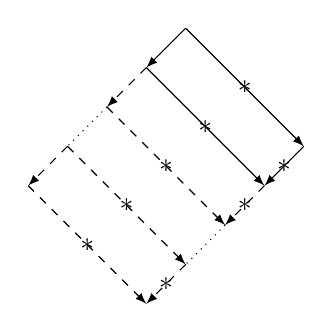
\begin{tikzpicture}[scale=0.5]
	\draw [-latex] (3,3) -- (2,2)  ;
	\draw [-latex] (3,3) --node{$*$} (6,0)  ;
	\draw [-latex] (2,2) --node{$*$} (5,-1)  ;
	\draw [-latex] (6,0) --node{$*$} (5,-1)  ;

	\draw [-latex, dashed] (2,2) -- (1,1) ;
	\draw [dotted] (1,1) -- (0,0) ;
	\draw [-latex, dashed] (0,0) -- (-1,-1) ;

	\draw [-latex, dashed] (1,1) --node{$*$}  (4,-2) ;
	\draw [-latex, dashed] (0,0) -- node{$*$} (3,-3) ;
	\draw [-latex, dashed] (-1,-1) -- node{$*$} (2,-4) ;

	\draw [-latex, dashed] (5,-1) -- node{$*$} (4,-2) ;
	\draw [dotted] (4,-2) -- (3,-3) ;
	\draw [-latex, dashed] (3,-3) -- node{$*$} (2,-4) ;
\end{tikzpicture}
\end{center}

\item L'idée de la démonstration est simple : supposons $M \stackrel{\Delta}{\rightarrow} M_1  $ où
$\Delta$ est un redex de $M$. Si dans la réduction $M\twoheadrightarrow M_2$, on garde la trace de ce qui se passe
sur $\Delta$, alors en réduisant tous les résidus de $M_2$, on obtiendra $M_3$.
\end{enumerate}

\subsection{La restriction $\Lambda '$ du $\lambda$-calcul}
Pour tracer les redex uniquement à réduire, on introduit $\Lambda '$, une restriction du $\lambda$-calcul.


$\Lambda '$ est définie de manière inductive comme ci-dessous comme le $\lambda$-calcul avec en addition
l'expression $((\lambda _i x.M)N)$ pour $i \in \mathbb{N}$
Ainsi, nous marquons par un indice $i$ le redex que nous voulons tracer.
Nous définissons également la réduction $\beta '$  qui contient la réduction $\beta$ et y ajoute 
$(\lambda_i x.M)N \rightarrow M [x:=N]$

Enfin, nous ajoutons la fonction $\phi$ qui réduit uniquement les redex indicés, et non les autres.
$$\phi ((\lambda _i x.P)Q) \equiv \phi (P) [x:=\phi(Q)]$$

Nous utilisons les notations $M\stackrel{\shortparallel }{\longrightarrow} N$
et $M\stackrel{\phi } {\longrightarrow}N$

Le pouvoir réducteur de $\beta '$ est le même que $\beta$.
En outre, on a la propriété suivante : si $M \stackrel{\beta '}{\twoheadrightarrow} N$,
alors   $\phi(M) \stackrel{\beta}{\longrightarrow} \phi (N)$ 

\subsection{La démonstration}
Nous présentons ici la démonstration détaillée dans \cite{baren_bible}.

\begin{enumerate}
	\item Hypothèses: $M\stackrel{\beta}{\twoheadrightarrow} N$ et
                    $M\stackrel{\beta}{\rightarrow} M'$        
       \item Cherchons à prouver qu'il existe $N'$ tel que  $N\stackrel{\beta}{\twoheadrightarrow} N'$ 
et  $M' \stackrel{\beta}{\twoheadrightarrow} N'$ 
        \item $M'$ est le résultat de la contraction du redex $\Delta$ dans $M$. Soit $\tilde{M} \in \Lambda '$
        obtenu de $M$ en indexant $\Delta$. Alors, $ \tilde{M} \stackrel{\shortparallel}{\rightarrow} M$ et 
       $ \tilde{M} \stackrel{\phi}{\rightarrow} M'$ 
       \item Nous obtenons, l'existence d'un $\tilde{N}$ par $\tilde{M}\stackrel{\beta '}\twoheadrightarrow \tilde{N}$
       \item Nous obtenons aussi l'existence d'un $N'$ tel que $\tilde{N} \stackrel{\phi}{\twoheadrightarrow} N'$
       et $N \stackrel{\beta}{\twoheadrightarrow} N'$
       \item Nous avons de même $M' \stackrel{\beta}{\twoheadrightarrow} N'$
       \item Nous avons bien trouvé notre terme confluent $N'\ \  \square $

\end{enumerate}

\subsection{Un exemple}
\begin{enumerate}
	\item Soit $M \equiv (\lambda x.xx)((\lambda y.z)w)$ , nous avons 
	$M \stackrel{\beta}{\rightarrow} N' \equiv (\lambda x.xx)z$ et $M \stackrel{\beta}{\rightarrow} N \equiv ((\lambda y.z)w)((\lambda y.z)w)$
       \item Cherchons  $N'$ tel que  $N\stackrel{\beta}{\twoheadrightarrow} N'$ 
et  $M' \stackrel{\beta}{\twoheadrightarrow} N'$ 
	\item  Soit le redex $\Delta$ de $M$ tel que $\Delta \equiv ((\lambda y.z)w)$, alors $\tilde{M} \equiv (\lambda x.xx)((\lambda_1 y.z)w)$
	Nous avons $\tilde{M}  \stackrel{\phi}{\rightarrow} M' \equiv (\lambda x.xx)z$
	\item $\tilde{N}$ est obtenu de la même manière que $N$, mais en marquant les résidus de $\Delta$ :
	 $\tilde{N} \equiv  ((\lambda _1 y.z)w)((\lambda _1 y.z)w)$

	 \item  Nous réduisons maintenant les résidus de $\tilde{N}$ pour obtenir
	  $\tilde{N}  \stackrel{\phi}{\twoheadrightarrow} zz$ \\
	  Aussi, nous avons bien également $N \stackrel{\beta}{\twoheadrightarrow} zz$

	 \item Nous avons également $M' \equiv (\lambda x.xx)z \stackrel{\beta}{\rightarrow} zz$
	 \item Ainsi $N' \equiv zz$
\end{enumerate}

\subsection{La $\beta$-réduction parallèle}
Une autre méthode de démonstration de la confluence repose sur l'introduction d'une nouvelle relation $\beta _\parallel $.
Cette relation va permettre la réduction simultanée de plusieurs redex du $\lambda$-terme.

\begin{definition}
	La $\beta _\parallel$ réduction repose sur les 4 règles suivantes:
	\begin{enumerate}
		\item  
		$ x \Rightarrow_\beta  x $
		\item 
		$ \lambda x.M \Rightarrow_\beta  \lambda x.M' , si\ M \Rightarrow_\beta  M' $
		\item 
		$ MN \Rightarrow_\beta  M' N' , \ si\ M  \Rightarrow_\beta  M' 
		                                               \ et\ N  \Rightarrow_\beta  N'$
		\item 
		$ (\lambda x.M)N \Rightarrow_\beta M'[x:=N'] , \ si\ M \Rightarrow_\beta  M' 
		                                               \ et\ N  \Rightarrow_\beta N'$
	\end{enumerate}

\end{definition}
On peut démontrer par induction que cette relation $\beta _\parallel$ respecte la propriété du diamant : si
$M \Rightarrow M_1,M_2$, alors $\exists N$ tel que $M_1,M_2  \Rightarrow N$.

Cependant, nous allons encore plus simplement montrer qu'il existe un $M^*$ tel que si $M  \Rightarrow N  \forall N$, alors
$N  \Rightarrow M^*$. Ce $M^*$ sera indépendant de $N$.
L'idée est que le terme $M^*$ sera obtenu en réduisant simultanément tous les redex présents dans $M$.


Soit la fonction $\mathcal{G}$, tel que 
\begin{align}
	\mathcal{G}(x)&=x \\
	\mathcal{G}(\lambda x.M) &= \lambda x.(\mathcal{G}(M)) \\
	\mathcal{G}(MN)&= \mathcal{G}(M)\mathcal{G}(N), \ si\ M \neq \lambda x.M_1 \\
	 \mathcal{G}((\lambda x.M)N) &= \mathcal{G}(M)[x:=\mathcal{G}(N)]  
\end{align}
Nous pouvons montrer que si $M  \Rightarrow _\beta N, \forall N$, alors
$N  \Rightarrow  _\beta \mathcal{G}(M)$.
Par induction sur la relation $M  \Rightarrow _\beta N$  :
 \begin{enumerate}
	\item si $M \equiv x$, alors $N \equiv x \equiv \mathcal{G}(x)$

	\item si $M \equiv \lambda x.M_1$, alors $N \equiv \lambda x.N_1$, avec $M_1  \Rightarrow _\beta N_1$. 
	Par récurrence, $M_1  \Rightarrow _\beta \mathcal{G}(M_1)$, donc $M  \Rightarrow _\beta \lambda x.\mathcal{G}(M)_1 \equiv
	\mathcal{G(M)}$

	\item si $M\equiv (M_1 M_2)  \Rightarrow _\beta  N $, alors $N \equiv N_1 N_2$ 
	avec $M_1 \Rightarrow _\beta N_1$ et  $M_2 \Rightarrow _\beta N_2$ , alors nous avons
	 $N_1 N_2 \Rightarrow _\beta \mathcal{G}(N_1) \mathcal{G}(N_2) \equiv \mathcal{G}(M)$

	 \item si $M\equiv ((\lambda x.M_1)M_2) \Rightarrow _\beta N$, alors 2 sous-cas à considérer :
	 \subitem 
	      si $N \equiv (\lambda x.N_1)N_2$, alors $N \Rightarrow _\beta \mathcal{G}(M_1)[x:=\mathcal{G}(M_2)] \equiv \mathcal{G}(M)$
	 \subitem 
	      si $N \equiv N_1[x:=N_2]$, alors $N \Rightarrow _\beta \mathcal{G}(M_1)[x:=\mathcal{G}(M_2)] \equiv \mathcal{G}(M)$ 


\end{enumerate}


\section{La $\beta$-réduction faible avec appel par valeur}
Dans un langage fonctionnel comme \textsc{Scheme} ou \textsc{ML}, il est important de noter que contrairement au $\lambda$-calcul, le corps de la lambda n'est pas \'{e}valu\'{e}. 
On parle de $\beta$-réduction faible.  
Autrement dit, la règle suivante n'est pas utilisée:
$$\mathbf{(abstraction)} : \frac{M \rightarrow M_1}{ \lambda x.M \rightarrow (\lambda x.M_1)}$$
Nous pourrons utiliser cette absence d'\'{e}valuation du corps 
des lambda expressions pour geler l'\'{e}valuation de nos expressions : \verb+(delay exp) = (lambda () exp)+ 

L'appel par valeur signifie que les arguments sont évalué en premier. Les règles d'inférence appliquées sont donc dans cet ordre:

$$
\quad \mathbf{(1)} : \frac{N \rightarrow N_1}{(M N) \rightarrow (M N_1)}
\quad \mathbf{(2)} : \frac{M \rightarrow M_1}{(M N) \rightarrow (M_1 N)}
\quad \mathbf{(3)} : \frac{}{((\lambda x.M)N) \rightarrow M[x \leftarrow N]} 
$$

Voici la fonction ML qui implémente cet ordre:
\begin{Verbatim}
let rec reduc1Valeur terme =
  match terme with
  | Var x -> raise IRREDUCTIBLE
  | Lam (x, m) -> raise IRREDUCTIBLE
  | App (n, m) ->
      (try App (n, (reduc1Valeur m))
       with
       | IRREDUCTIBLE ->
           (try App ((reduc1Valeur n), m)
            with
            | IRREDUCTIBLE ->
                (try betaReducRedex terme
                 with | NOTREDEX -> raise IRREDUCTIBLE)))
\end{Verbatim}

Par exemple, nous aurons les réductions successives suivantes: 

\begin{itemize}
\item réduction normale, qui aboutit toujours à la forme irréductibre
$$ (\lambda x.y) ((\lambda x.xx) (\lambda x.xx)) \rightarrow_\beta y $$ 

\item réduction par valeur 
$$
\begin{array}{ccc}
 (\lambda x.y)((\lambda x.xx) (\lambda x.xx)) &  \rightarrow_\beta  & (\lambda x.y)((\lambda x.xx) (\lambda x.xx))\\ 
 & \rightarrow_\beta  & (\lambda x.y)((\lambda x.xx) (\lambda x.xx)) \\
 &\rightarrow_\beta  & (\lambda x.y)((\lambda x.xx) (\lambda x.xx))) \\
 & \rightarrow_\beta  & \ldots \\
\end{array}
$$
\end{itemize}

\section{Récursivité et points fixes} 

What else is a loop but a way of representing an endless process in a finite way?
\cite{god}


\begin{center}
 \begin{tabular}{cc}
	\parbox[c]{0.3\textwidth}{
\includegraphics[width=0.3\textwidth]{DrawingHands.jpg}}
  & \hspace{0.5cm}
   $\sqrt{2} = 1 + \frac{1}{1+\sqrt{2}} $  \\
 \end{tabular}
\end{center}

\subsection{Le point fixe du $\lambda$-calcul} %%

En analyse, le point fixe d'une fonction $f$ est sa valeur $x$ telle que $f(x)=x$

Cela permet de d\'{e}finir $x$ en fonction de lui-m\^{e}me.

Cette simple expression $x=f(x)$ est finalement tr\`{e}s \'{e}trange et d\'{e}routante.
C'est la force de la r\'{e}cursivit\'{e} : $x=f(f(f(f(f(f\ldots (x)\ldots))))))$

Un exemple est la valeur $\sqrt{2}$ exprim\'{e}e sous forme d'une fraction continue,
expression trouv\'{e}e je crois par Euler.
Je la d\'{e}cris ci-dessous  pour le plaisir d'\'{e}crire (et lire) de belles formules math\'{e}matiques en \LaTeX
\cite{lamport1994latex}
$$
\sqrt{2} = 1+\sqrt{2} -1
= 1+ \frac{(\sqrt{2} -1)(\sqrt{2} +1)}{\sqrt{2} +1}
= 1 + \frac{1}{1+\sqrt{2}}
$$


\begin{tikzpicture}
	\draw[->] (-1, 0) -- (3, 0) node[right] {$x$};
	\draw[->] (0, -1) -- (0, 3) node[above] {$y$};
	\draw[domain=-0.5:3, smooth, variable=\x, blue] plot (\x, {1 + 1 / (1+ \x) }) node [right] {$y=1 + \frac{1}{1+x} $};
	\draw[domain=-1:3, smooth, variable=\x, red] plot (\x, {\x}) node [right] {$y=x$};
	\draw [dotted] (1.4142,0) node[below]{$\sqrt{2}$}  --(1.4142,1.4142)  ;
	\draw [dotted] (0,1.4142) node[left] {$\sqrt{2}$}  --(1.4142,1.4142) ;
	
	\node [draw,text width=6cm] at(10,1.5) {\[
		\sqrt{2} = 1 + \cfrac{1}{2
		+ \cfrac{1}{2
		+ \cfrac{1}{2
		+ \cfrac{1}{2
		+ \cfrac{1}{ \ddots
		} } } } } \] } ;
\end{tikzpicture} 



En posant $ f(x) = 1 + \frac{1}{1+x} $, la résolution de l'équation $x=f(x)$ nous permet
de calculer la valeur de $\sqrt{2}$. Nous utilisons aussi le fait que $\sqrt{2}$ est 
un point fixe attractif de notre fonction $f$. C'est-à-dire qu'il existe un \textit{voisinage} de 
$\sqrt{2}$ tel que la suite $ x_0,f(x_0),f(f(x_0)),f(f(f(x_0))),\dots $ converge vers $\sqrt{2}$


En \textsc{Ocaml}, la fonction qui it\`{e}re cette fraction continue peut être codée comme suit. 
Nous partons ici de $x_0 =1$. La fraction continue converge très rapidement.
\begin{Verbatim}
let rec square2 iter =
	if (iter = 1) then 1.
	else  1. +. ( 1. /. ( 1. +. square2 (iter - 1)));;
val square2 : int -> float = <fun>

# square2 30 ;;
- : float = 1.4142135623730951

# sqrt 2. ;;
- : float = 1.41421356237309512.

\end{Verbatim}


En $\lambda $-calcul, de manière très surprenante, il s'avère que tout terme a un point fixe !
Nous avons un combinateur\footnote{Un combinateur est un $\lambda$-terme comprenant uniquement 
des variables li\'{e}es} qui nous permet de calculer le point fixe de n'importe quel $\lambda $-terme.
Ce combinateur s'appelle $Y$ . Il est défini par $$ Y=  \lambda f.(\lambda x.f(x x))(\lambda x.f(x x)) $$

Ce n'est pas le seul combinateur de point fixe. Voici un autre d\^{u} \`{a} Turing :
 $$\Theta = (\lambda x. \lambda y. (y (x x y))) (\lambda x. \lambda y. (y (x x y)))$$

Voici l'arbre syntaxique de $Y$:
\begin{center}
\begin{tikzpicture}[level distance=1.5cm,
level 1/.style={sibling distance=5cm},
level 2/.style={sibling distance=3cm},
level 3/.style={sibling distance=1.5cm},
level 4/.style={sibling distance=1.5cm}, scale=0.6]
\node {$\lambda$} child { node{f} } child {node {@} child { node {$\lambda$} child
{ node{x} } child {node {@} child { node {f }}  child {node {@} child { node {x }}
child {node {x }} } } }  child {node {$\lambda$} child { node{x} } child
{node {@} child { node {f }}  child {node {@} child { node {x }}  child {node {x }} } } } } ;
\end{tikzpicture}
\end{center}
Quel que soit le terme $M$, nous aurons  $(YM) = _\beta M(YM)$



Essayons ceci avec notre notre fonction \verb+fullReduc+  en CAML.
Réduisons $YM$ :

$$
\begin{array}{l}
\lambda f . (\lambda x . (f (x x))) (\lambda x . (f (x x))) M \\
\rightarrow _\beta (\lambda x . (M (xx)))(\lambda x . (M(xx))) \\
\rightarrow _\beta  (M(\lambda x . (M(xx)))(\lambda x . (M(xx))))  \triangleright [2] \\
\rightarrow _\beta  (MM(\lambda x . (M(xx)))(\lambda x . (M(xx)))) \\
\rightarrow _\beta  (MMM(\lambda x . (M(xx)))(\lambda x . (M(xx)))) \\
\rightarrow _\beta  (MMMM(\lambda x . (M(xx)))(\lambda x . (M(xx)))) \\
\rightarrow _\beta  \ldots
\end{array}
$$


La deuxième $\beta$-r\'{e}duction est bien \'{e}gale \`{a} $M (Y M)$
Nous voyons ici le mécanisme d'appel récursif à M. 

Détaillons cela avec une fonction exprimée en pseudo-code d'un $\lambda$-calcul étendu.
Nous nous inspirons pour cela du très bon article de wikipedia \url{https://en.wikipedia.org/wiki/Lambda_calculus}.


Soit $M = (\lambda f \lambda n .(if\ n=0\ then\ 1\ else\ n*f(n-1)))$
$$
\begin{array}{lll}
(YM)\ 4 & \rightarrow _\beta & M (YM)\ 4 \\
& \rightarrow _\beta & (\lambda f \lambda n .(if\ n=0\ then\ 1\ else\ n*f(n-1))) (YM)\ 4 \\
& \rightarrow _\beta & (\lambda  n . (if\ n=0\ then\ 1\ else\ n*((YM) (n-1))))\ 4 \\
& \rightarrow _\beta & (if\ 4=0\ then\ 1\ else\ 4*((YM)\ (4-1))) \\
& \rightarrow _\beta & 4 * ((YM)\ 3) \\
& \rightarrow _\beta & 4 * (M(YM)\ 3) \\
& \vdots & \\
& \rightarrow _\beta & 4 * 3 * 2 * 1 
\end{array}
$$

Ici encore, nous avons utilisé la stratégie de $\beta$-réduction normale. 
Mais avec une réduction par valeur, le terme en argument $(YM)$ aura été réduit indéfiniment en $M(M(M(M(M\ldots YM)\ldots)))$,
sans réduire le redex $Mx$


En utilisant notre programme OCAML, voyons cela avec en prenant $M = \lambda a. (\lambda b . b) $ :

\verb+# betaNormal ym ;;+
$$
\begin{array}{lll}
 & (\lambda f . (\lambda x . (f(xx))\lambda x . (f(xx)))\lambda a . \lambda b . b) &  \\
 \rightarrow _\beta & (\lambda x . (\lambda a . \lambda b . b(xx))\lambda x . (\lambda a . \lambda b . b(xx))) &\triangleright [2]  \\
 \rightarrow _\beta & (\lambda a . \lambda b . b(\lambda x . (\lambda a . \lambda b . b(xx))\lambda x . (\lambda a . \lambda b . b(xx))))  &\triangleright [3]  \\
 \rightarrow _\beta & \lambda b . b &  \\
\end{array}
$$

\verb+# betaValeur ym ;;+
$$
\begin{array}{lll}
 & (\lambda f . (\lambda x . (f(xx))\lambda x . (f(xx)))\lambda a . \lambda b . b)  &  \\
\rightarrow _\beta & (\lambda x . (\lambda a . \lambda b . b(xx))\lambda x . (\lambda a . \lambda b . b(xx))) & \triangleright [2]  \\
\rightarrow _\beta & (\lambda a . \lambda b . b(\lambda x . (\lambda a . \lambda b . b(xx))\lambda x . (\lambda a . \lambda b . b(xx)))) & \triangleright [3] \\
\rightarrow _\beta & (\lambda a . \lambda b . b(\lambda a . \lambda b . b(\lambda x . (\lambda a . \lambda b . b(xx))\lambda x . (\lambda a . \lambda b . b(xx)))))  & \\
\rightarrow _\beta & (\lambda a . \lambda b . b(\lambda a . \lambda b . b(\lambda a . \lambda b . b(\lambda x . (\lambda a . \lambda b . b(xx))\lambda x . (\lambda a . \lambda b . b(xx)))))) &  \\
\rightarrow _\beta & (\lambda a . \lambda b . b(\lambda a . \lambda b . b(\lambda a . \lambda b . b(\lambda a . \lambda b . b(\lambda x . (\lambda a . \lambda b . b(xx))\lambda x . (\lambda a . \lambda b . b(xx)))))))  & \\
\end{array}
$$
Les étapes  $\triangleright [2]$ et $\triangleright [3]$ sont bien les mêmes sur les deux stratégies. 
Puis la $\beta$-réduction par valeur va continuer à réduire l'argument
$(YM)$, là où la $\beta$-réduction normale va d'abord réduire le redex $Mx$

Avec la réduction par valeur, il nous faut donc utiliser un autre combinateur de point fixe\footnote{Nous insistons 
là-dessus car nous rappelons que les interprètes \textsc{MiniScheme} et \textsc{MiniML} que nous implémenterons utiliseront la $\beta$-réduction faible par valeur.}
 que nous appelerons $Z$ 
$$Z = \lambda f.(\lambda x.f(\lambda v.xxv))(\lambda x.f(\lambda v.xxv)) $$

On constate que Z est  $\eta$-équivalent à $Y$. Nous rappelons la définition suivante:


\begin{definition}
	
Les termes $(\lambda x.Mx)$ et M sont $\eta$-équivalents. On écrira $(\lambda x.Mx) =_\eta M$

En ML, nous pouvons par exemple dire que \verb+ let g x = f x+ est $\eta$-équivalent à \verb+ let g = f+
\end{definition}


Appliquons à nouveau notre exemple avec ce combinateur $Z$ appliqué à $M=\lambda a. \lambda b. b$:

\verb+# betaValeur zm ;;+
$$
\begin{array}{ll}
& ((\lambda f . ((\lambda x . (f(\lambda v . ((xx)v))))(\lambda x . (f(\lambda v . ((xx)v))))))(\lambda a . (\lambda b . b))) \\
\rightarrow _\beta &  ((\lambda x . ((\lambda a . (\lambda b . b))(\lambda v . ((xx)v))))(\lambda x . ((\lambda a . (\lambda b . b))(\lambda v . ((xx)v))))) \\
\rightarrow _\beta &  ((\lambda a . (\lambda b . b))(\lambda v . (((\lambda x . ((\lambda a . (\lambda b . b))(\lambda v . ((xx)v))))(\lambda x . ((\lambda a . (\lambda b . b))(\lambda v . ((xx)v)))))v))) \\
\rightarrow _\beta &  (\lambda b . b)
\end{array}
$$

Nous avons le même réultat et les même étapes de réduction avec \verb+betaNormal zm ;;+


En SCHEME, nous pourrons implémenter ce combinateur $Z$ :
\begin{Verbatim}
(define Z
 (lambda(f)
   (lambda (x) (lambda(v) ((f (x x) v))))
   (lambda (x) (lambda(v) ((f (x x) v))))))
\end{Verbatim}

En ML, le typage ne nous permettra pas de coder un combinateur comme $Y$ ou $Z$.

Essayons cependant d'écrire:

\begin{Verbatim}

# let rec fix f = f (fix f) ;;
val fix : ('a -> 'a) -> 'a = <fun>

let factabs fact = function
  | 0 -> 1
  | n -> n * fact (n - 1) ;;

val factabs : (int -> int) -> int -> int = <fun>
# (fix factabs) 5 ;;
Stack overflow during evaluation (looping recursion?).
\end{Verbatim}
ML est bien un langage \textit{strict}: les arguments d'une fonction sont évalués en premier 
comme on l'a vu dans la $\beta$-réduction faible avec appel par valeur.


Pour éviter la boucle infinie $f(f\ldots(f (fix f))\ldots)$, 
une astuce que j'ai pu lire est d'introduire une variable supplémentaire:

\begin{Verbatim}
# let rec fix f x = f (fix f) x ;;
val fix : (('a -> 'b) -> 'a -> 'b) -> 'a -> 'b = <fun>
# (fix factabs) 5 ;;
- : int = 120
\end{Verbatim}
Ici aussi, le mécanisme de la ``$\eta$-expansion'' est utilisé.
Je ne peux reproduire cela en SCHEME:

\begin{Verbatim}
(define factabs
  (lambda (f)
    (lambda (n)
      (if (eq? n 0)
          1
          (* n (f (- n 1)))))))

(define y
  (lambda (f x)
    (f (y f) x)))

(y factabs 5)
=> y: arity mismatch; the expected number of arguments does not match 
  expected: 2
  given: 1
\end{Verbatim}

\subsection{La diagonale de Cantor} %%
 A la différence du $\lambda$-calcul où tout terme a un point fixe, la recherche de point fixe
peut amener à des situations paradoxales.
Voyons cela avec le théorème  de Cantor.


Ce théorème nous dit qu'il n'y a pas de fonction surjective 
$f: \mathbb{N} \rightarrow ( \mathbb{N} \rightarrow \mathbb{B}) $.
Autrement dit, le cardinal des parties de $\mathbb{N}$ est strictement plus grand que le cardinal de $\mathbb{N}$.
Démontrons cela. \\
Soient $X_0, X_1, \ldots, X_n$ les parties de $\mathbb{N}$  \\
Soit $f(m,n) = true$ si $m \in X_n$ et $false$ sinon. \\
Soit $g :\mathbb{B} \rightarrow \mathbb{B}$ la fonction sans point fixe telle que $g(false)=true$ et $g(true)=false$. \\
Considérons la fonction $h: \mathbb{N} \rightarrow \mathbb{B}$ telle que $h(x) = g(f(x,x))$
Supposons $f$ surjective donc $\exists a, f(a)= h \Leftrightarrow  f(a,a) = h(a) = g(f(a,a))$ 
Cela est impossible car $g$ n'admet pas de point fixe par définition.

Ainsi $f$ n'est pas surjective. \qedsymbol
\vspace{0.5cm}

Voici la représentation matricielle de la fonction $f(x,y)$. Les valeurs $true$ et $false$ sont représentées par $1$ et $0$.
La colonne est la valeur de $x$ et la ligne est la valeur de $y$.

\[
\begin{bmatrix}
 0 & 1 & 2 & 3 & 4 & 5 & 6 & 7 &  ... &     \\ 
 \mathbf{1} & 0 & 0 & 1 & 0 & 1 & 0 & 1 &  ... &   X_0 \\
 0 & \mathbf{0} & 0 & 1 & 0 & 0 & 0 & 0 &  ... &   X_1 \\
 1 & 0 & \mathbf{1} & 1 & 1 & 1 & 1 & 0 &  ... &   X_2 \\
 1 & 0 & 0 & \mathbf{1} & 0 & 1 & 0 & 0 &  ... &   X_3 \\
 0 & 0 & 0 & 1 & \mathbf{0} & 1 & 0 & 0 &  ... &   X_4 \\
 0 & 0 & 0 & 0 & 0 & \mathbf{1} & 0 & 1 &  ... &   X_5 \\
 0 & 0 & 0 & 1 & 1 & 0 & \mathbf{1} & 0 &  ... &   X_6 \\
 0 & 0 & 0 & 0 & 0 & 0 & 0 & \mathbf{0} &  ... &   X_7 \\
   &   &   &   &   & \vdots &  &  &\ddots  \\
\end{bmatrix}
\Rightarrow_{g(f(x,x))}
\begin{bmatrix}
 0 & 1 & 2 & 3 & 4 & 5 & 6 & 7 &  ... &     \\ 
 \mathbf{0} & 0 & 0 & 1 & 0 & 1 & 0 & 1 &  ... &   X_0 \\
 0 & \mathbf{1} & 0 & 1 & 0 & 0 & 0 & 0 &  ... &   X_1 \\
 1 & 0 & \mathbf{0} & 1 & 1 & 1 & 1 & 0 &  ... &   X_2 \\
 1 & 0 & 0 & \mathbf{0} & 0 & 1 & 0 & 0 &  ... &   X_3 \\
 0 & 0 & 0 & 1 & \mathbf{1} & 1 & 0 & 0 &  ... &   X_4 \\
 0 & 0 & 0 & 0 & 0 & \mathbf{0} & 0 & 1 &  ... &   X_5 \\
 0 & 0 & 0 & 1 & 1 & 0 & \mathbf{0} & 0 &  ... &   X_6 \\
 0 & 0 & 0 & 0 & 0 & 0 & 0 & \mathbf{1} &  ... &   X_7 \\
   &   &   &   &   & \vdots &  &  &\ddots  \\
\end{bmatrix}
\]


\vspace{0.5cm}

Voici la démonstration formelle en COQ.
\\


\begin{coqdoccode}
\coqdocnoindent
\coqdockw{Require} \coqdockw{Import} \coqdocvar{Bool}.\coqdoceol
\coqdocemptyline
\coqdocnoindent
\coqdockw{Section} \coqdocvar{Cantor}.\coqdoceol
\coqdocemptyline
\coqdocnoindent
\coqdockw{Lemma} \coqdocvar{negb\_prop} : \coqdockw{\ensuremath{\forall}} \coqdocvar{a}:\coqdocvar{bool}, \coqdocvar{negb} \coqdocvar{a} =\coqdocvar{a} \ensuremath{\rightarrow} \coqdocvar{False}.\coqdoceol
\coqdocnoindent
\coqdockw{Proof}.\coqdoceol
\coqdocindent{2.00em}
\coqdoctac{intros}.\coqdoceol
\coqdocindent{2.00em}
\coqdoctac{unfold} \coqdocvar{negb} \coqdoctac{in} \coqdocvar{H}.\coqdoceol
\coqdocindent{2.00em}
\coqdoctac{induction} \coqdocvar{a}. \coqdoctac{inversion} \coqdocvar{H}. \coqdoctac{inversion} \coqdocvar{H}.\coqdoceol
\coqdocnoindent
\coqdockw{Qed}.\coqdoceol
\coqdocemptyline
\coqdocnoindent
\coqdockw{Definition} \coqdocvar{surjective} \{\coqdocvar{X}:\coqdockw{Type}\} (\coqdocvar{f} : \coqdocvar{nat} \ensuremath{\rightarrow} \coqdocvar{X}) : \coqdockw{Prop} := \coqdockw{\ensuremath{\forall}} \coqdocvar{y}, \coqdoctac{\ensuremath{\exists}} \coqdocvar{x}, \coqdocvar{f} \coqdocvar{x} = \coqdocvar{y}.\coqdoceol
\coqdocemptyline
\coqdocnoindent
\coqdockw{Theorem} \coqdocvar{cantor} : \ensuremath{\lnot} \coqdoctac{\ensuremath{\exists}} \coqdocvar{f} : \coqdocvar{nat} \ensuremath{\rightarrow} \coqdocvar{nat} \ensuremath{\rightarrow} \coqdocvar{bool}, \coqdocvar{surjective} \coqdocvar{f}.\coqdoceol
\coqdocnoindent
\coqdockw{Proof}.\coqdoceol
\coqdocindent{2.00em}
\coqdoctac{intros} [\coqdocvar{f} \coqdocvar{SURJ}].\coqdoceol
\coqdocindent{2.00em}
\coqdoctac{pose} (\coqdocvar{g} := \coqdockw{fun} \coqdocvar{b} \ensuremath{\Rightarrow} \coqdocvar{negb} \coqdocvar{b} ).\coqdoceol
\coqdocemptyline
\end{coqdoccode}
soit $h$ la diagonalisation négative de la mort 

\begin{coqdoccode}
\coqdocindent{2.00em}
\coqdoctac{pose} (\coqdocvar{h} := \coqdockw{fun} \coqdocvar{x} \ensuremath{\Rightarrow} \coqdocvar{g} (\coqdocvar{f} \coqdocvar{x} \coqdocvar{x})).\coqdoceol
\coqdocemptyline
\end{coqdoccode}
on applique l'hypothèse de surjection de $f$ sur $h$

 \begin{coqdoccode}
\coqdocindent{2.00em}
\coqdoctac{destruct} (\coqdocvar{SURJ} \coqdocvar{h}) \coqdockw{as} [\coqdocvar{x} \coqdocvar{B}].\coqdoceol
\coqdocindent{2.00em}
\coqdoctac{assert} (\coqdocvar{C}: \coqdocvar{h} \coqdocvar{x} = \coqdocvar{f} \coqdocvar{x} \coqdocvar{x}).\coqdoceol
\coqdocindent{2.00em}
\{\coqdoceol
\coqdocindent{4.00em}
\coqdoctac{rewrite} \coqdocvar{B}. \coqdoctac{reflexivity}.\coqdoceol
\coqdocindent{2.00em}
\}\coqdoceol
\coqdocindent{2.00em}
\coqdoctac{unfold} \coqdocvar{h} \coqdoctac{in} \coqdocvar{C}.\coqdoceol
\coqdocindent{2.00em}
\coqdoctac{unfold} \coqdocvar{g} \coqdoctac{in} \coqdocvar{C}.\coqdoceol
\coqdocindent{2.00em}
\coqdoctac{apply} \coqdocvar{negb\_prop} \coqdoctac{in} \coqdocvar{C}.\coqdoceol
\coqdocindent{2.00em}
\coqdoctac{assumption}.\coqdoceol
\coqdocnoindent
\coqdockw{Qed}.\coqdoceol
\coqdocemptyline
\coqdocnoindent
\coqdockw{End} \coqdocvar{Cantor}.\coqdoceol
\end{coqdoccode}

Nous pourrons nous reférer à l'ouvrage de Jean-Yves Girard, \textit{Le Point Aveugle}
\cite{girard}

La construction ci-dessus appliquée sur le $\lambda$-calcul permet de mettre en évidence de 
manière constructive que tout $\lambda$-terme a un point fixe.
Considérons la fonction $f \equiv \lambda xy.xy$, l'application $xy$ dénote $x \in y$.
Soit $g$ une fonction quelconque dont on recherche un point fixe.
Considérons $h\equiv \lambda x.g(f (x x))=\lambda x.g(x x)$, alors $h h$ est 
le point fixe recherché car :
$$
hh=(\lambda x.g(xx))(\lambda x.g(xx))=g(\lambda x.g(xx)(\lambda x.g(xx)))=g(hh)
$$

\subsection{Le point fixe logique et le théorème d'incomplétude de Gödel} %%
Il y a une similitude forte entre le point fixe du $\lambda$-calcul et le point fixe \textit{logique}. Voyons cela.

Nous ne décrirons pas le mécanisme de codage. 
Nous utiliserons les fonctions suivantes :
\begin{align*}
\ulcorner t  \urcorner :& \  terme \rightarrow terme \hspace{1.3cm} \text{la fonction qui donne le code syntaxique d'un terme}\\
\#  t :& \  terme \rightarrow \mathbb{N} \hspace{2cm} \text{la fonction qui donne le code numérique d'un terme}\\
\overline{  n } :& \  \mathbb{N} \rightarrow terme \hspace{2cm}  \text{la fonction qui transforme un code numérique
 en code syntaxique}
\end{align*}

On notera ainsi $\ulcorner t \urcorner$, le terme $\overline{n}$  si 
$\# t =n$ . 


\begin{theoreme}[Le point fixe logique]
	Soit $T$ une théorie permettant de définir toutes les fonctions récursives.
	Soit $\psi$ une formule quelconque avec une variable libre. Il existe une proposition $\phi$ telle que
	$$ T \vdash \phi \leftrightarrow \psi (\ulcorner \phi\urcorner ) $$
\end{theoreme}
\begin{proof}
	Soit la fonction diagonale $d : \mathbb{N} \rightarrow \mathbb{N} $ définie par :
	$ d(n)= \# \chi _n(\overline{n})$ où $\chi_n$ est telle que $\# \chi =n$. Ainsi $d$ 
	est une fonction récursive et donc définissable dans notre théorie $T$. On a donc :
	$$T \vdash \forall y (\delta(\overline{n}, y)) \leftrightarrow y=\overline{d(n)} $$

	Soit la formule $\alpha$ telle que $\alpha (x)=\exists y (\delta(x,y) \land \psi(y))$
	, alors notre point fixe est $\phi = \alpha (\ulcorner \alpha \urcorner )$ \\
	En effet :

	\begin{align*}
	 T \vdash \phi & \leftrightarrow \alpha(\ulcorner \alpha \urcorner ) \\
	                 & \leftrightarrow \exists y\ (\delta( \ulcorner \alpha \urcorner , y) \land \psi (y)) \\
	                 & \leftrightarrow \exists y\ (y=\ulcorner \alpha(\ulcorner \alpha  \urcorner)\urcorner \land \psi (y)) \\
	                 & \leftrightarrow \psi (\ulcorner \alpha(\ulcorner \alpha \urcorner)\urcorner)  \\
	                 & \leftrightarrow \psi (\ulcorner \phi \urcorner ) \\
	\end{align*}
\end{proof}


La similitude avec le point fixe du $\lambda$-calcul est directe :
$$
\begin{array}{c|c}
 \phi \leftrightarrow \psi (\ulcorner \phi\urcorner ) & p = fp \\
 \delta(x,y) & \lambda x.xx \\
 \exists y (\delta(x,y) \land \psi(y)) & \lambda x.f (x x) \\
 \phi \equiv \alpha(\ulcorner \alpha \urcorner) & p \equiv (\lambda x.f(xx)) (\lambda x.f(xx)) \\
\end{array}
$$

\begin{theoreme}[Indécidabilité de l'arithmétique]
	Soit $T$ une théorique consistance telle que toutes les fonctions récursives
	y soient $T$-définissables, alors $T$ est essentiellement indécidable.
\end{theoreme}
\begin{proof}
        Soit la formule $th(\ulcorner x \urcorner)$ telle que :
	\begin{align*}
	T \vdash th(\ulcorner x \urcorner) \ &\text{ssi $x$ est un théorème de $T$} \\
	T \vdash \neg th(\ulcorner x \urcorner) \ &\text{ssi $x$ n'est pas un théorème de $T$} \\
	\end{align*}
	Reprenons le thèorème du point fixe :
	 $ T \vdash \phi \leftrightarrow \psi (\ulcorner \phi\urcorner ) $ et appliquons le à
	 la fonction $\neg th$.
	 
	 Nous avons alors l'existence d'un point fixe $G$ tel que
	  $$T \vdash G \leftrightarrow \neg th (\ulcorner G \urcorner ) $$ 

	  Nous avons la contradiction suivante : $T \vdash G$ ssi $T \vdash th(\ulcorner G \urcorner)$ par définition de $th$
	  et $T \vdash G$ ssi $T \vdash \neg th (\ulcorner G \urcorner)$ par construction de $G$
\end{proof}

\begin{theoreme}[Gödel, incomplétude de l'arithmétique]
	Toute théorie consistante et telle que toutes les fonctions récursives y soient définissables
	est incomplète.	
\end{theoreme}


\subsection{L'indécidabilité de la $\beta$-conversion} %%
Ce théorème repose encore sur l'existence d'un point fixe. 
Sa démonstration est ainsi toujours similaire au théorème d'incomplétude de Gödel ou au 
théorème de Rice.
\begin{theoreme}[point fixe du $lambda$-calcul]
	Pour tout $\lambda$-terme $F$, il existe un point fixe $X$ tel que 
	$F \ulcorner X \urcorner = X $ 
\end{theoreme}
\begin{proof}
Considérons les fonctions récursives $App$ et $Num$ telles que $App(\#M, \#N)=\#MN$	
et $Num(n)=\#\ulcorner M \urcorner $. Et considérons les fonctions $\lambda$-équivalentes 
$\mathbf{App}$ et $\mathbf{Num}$.

Alors, $\mathbf{App}\ulcorner M \urcorner \ulcorner N \urcorner = \ulcorner MN \urcorner$ et 
$\mathbf{Num}\ulcorner n \urcorner = \ulcorner \ulcorner n \urcorner \urcorner$

Soit $W \equiv \lambda x.F(\mathbf{App}\ x \ (\mathbf{Num}\ x))$, alors notre point fixe est
 $X\equiv W \ulcorner W \urcorner$

En effet,
\begin{align*}
 X=W\ulcorner W \urcorner &= F(\mathbf{App}\ulcorner W \urcorner (\mathbf{Num}\ulcorner W \urcorner)) \\
			  &= F \ulcorner W \ulcorner W \urcorner \urcorner \\
			  &= F \ulcorner X \urcorner
\end{align*}

\end{proof}

\begin{definition}[Ensembles récursivement séparables]
Deux ensembles $\mathcal{A}$ et $\mathcal{B}$ sont récursivement séparables ssi il existe un 
ensemble récursif $\mathcal{C}$	tel que $\mathcal{A} \subset \mathcal{C}$ et 
$\mathcal{B} \cap \mathcal{C} = \varnothing $
\end{definition}

\begin{definition}[Clôture d'un ensemble de $\lambda$-termes par $\beta$-conversion]
	Soit $\Lambda$ l'ensemble des $\lambda$-termes. Considérons $\mathcal{A} \subset  \Lambda$, 
	$\mathcal{A}$ est clos par égalité \textit{closed under equality} si :
	$$ \forall M, N \in \Lambda, (M \in \mathcal{A}  \ \text{et}\  M=_{\beta}N) \Rightarrow 
	                              N \in \mathcal{A}$$ 
\end{definition}

\begin{theoreme}[Indécidabilité de la $\beta$-conversion]
Soient deux ensembles $\mathcal{A}$ et $\mathcal{B}$ clos par $\beta$-conversion, alors 
$\mathcal{A}$ et $\mathcal{B}$ ne sont pas récursivement séparables.	
\end{theoreme}

\begin{proof}
	Soient $M_\mathcal{A} \in \mathcal{A}$ et  $M_\mathcal{B} \in \mathcal{B}$.
	Supposons l'existence de $\mathcal{C}$, un ensemble récursif et tel que 
	$\mathcal{A} \subset \mathcal{C}$ et $\mathcal{B} \cap \mathcal{C} = \varnothing$
	
	Soit $F$ la $\lambda$-fonction caractéristique de l'ensemble récursif $\mathcal{C}$,
	nous avons alors :
	\begin{align*}
		M \in \mathcal{C} \Rightarrow F \ulcorner M \urcorner = \ulcorner 0 \urcorner \\
		M \notin \mathcal{C} \Rightarrow F \ulcorner M \urcorner = \ulcorner 1 \urcorner \\
	\end{align*}
	
	Définissons $G \equiv \lambda x.\text{si\ zero}(Fx) \text{\ alors\ } M_\mathcal{B}
	\text{\ sinon\ } M_\mathcal{A}$

	D'après le théorème du point fixe, il existe $X$ tel que $G\ulcorner X \urcorner = X$,
	nous avons alors la contradiction suivante :
	\begin{align*}
		X \in \mathcal{C}, G \ulcorner X \urcorner = X = M_\mathcal{B} \Rightarrow X \notin \mathcal{C} \\
		X \notin \mathcal{C}, G \ulcorner X \urcorner = X = M_\mathcal{A} \Rightarrow X \in \mathcal{C} \\
	\end{align*}
\end{proof}
%%%%%%%%%%%%%%%%%%%%%%%%%%%%%%%%%%%%%%%%%%%%%%%%%%%%%%%%%%%%%%%%%%%%%%%%%%%%%%%%%%%%%%%%%%
%%%%%%%%%%%%%%%%%%%%%%%%%%%%%%%%%%%%%%%%%%%%%%%%%%%%%%%%%%%%%%%%%%%%%%%%%%%%%%%%%%%%%%%%%%
\section{Encoding. Les entiers \textit{Church} et les booléens en $\lambda$-calcul}
\subsection{Les entiers \textit{Church} }
Les entiers peuvent être représenté de la manière suivante:
$$
\begin{array}{l}
0 \equiv \lambda f.\lambda x.x \\
1 \equiv \lambda f.\lambda x.f x \\
2 \equiv \lambda f.\lambda x.f (f x) \\
3 \equiv \lambda f.\lambda x.f (f (f x)) 
\end{array}
$$

La fonction successeur se définira $SUCC \equiv \lambda n.\lambda f.\lambda x.f (n f x)$
Avec notre représentation ML: 

\verb+Lam("n", Lam("f", Lam("x",App(Var "f", App(App(Var "n", Var "f"), Var "x")))))+

Exécutons avec la stratégie normale, puis avec la stratégie de réduction faible par valeur:


\verb+# betaNormalPrint (App(succ, un)) ;;+
$$
\begin{array}{ll}
& (\lambda n . \lambda f . \lambda x . (f((nf)x))\lambda f . \lambda x . (fx))   \\
\rightarrow _\beta & \lambda f . \lambda x . (f((\lambda f . \lambda x . (fx)f)x))   \\
\rightarrow _\beta & \lambda f . \lambda x . (f(\lambda x . (fx)x))   \\
\rightarrow _\beta & \lambda f . \lambda x . (f(fx))   \\
& Exception: IRREDUCTIBLE.
\end{array}
$$

\verb+# betaValeurPrint (App(succ, un)) ;;+
$$
\begin{array}{ll}
& (\lambda n . \lambda f . \lambda x . (f((nf)x))\lambda f . \lambda x . (fx))   \\
\rightarrow _\beta & \lambda f . \lambda x . (f((\lambda f . \lambda x . (fx)f)x))   \\
& Exception: IRREDUCTIBLE.
\end{array} 
$$
Nous n'aboutissons pas au terme $\lambda f . \lambda x . (f(fx)) $ avec la stratégie par valeur. Nous voyons que le corps de la lambda
n'est pas évalué. Je suis cependant surpris car je pensais cette stratégie (même si appelée \textit{faible}) parvenait à calculer la
forme normale.

Nous pouvons écrire en OCAML la fonction qui convertit des entiers vers les terms \textit{Church}:
\begin{Verbatim}

let rec int2Church = function
	| 0 -> Lam("f", Lam("x", Var "x"))
	| n -> App(succ, int2Church (n-1))
\end{Verbatim}

\verb+# betaNormal (int2Church 3) ;;+
$$
\begin{array}{ll}
 & (\lambda n . \lambda f . \lambda x . (f((nf)x))(\lambda n . \lambda f . \lambda x . (f((nf)x))(\lambda n . \lambda f . \lambda x . (f((nf)x))\lambda f . \lambda x . x)))   \\
\rightarrow _\beta & \lambda f . \lambda x . (f(((\lambda n . \lambda f . \lambda x . (f((nf)x))(\lambda n . \lambda f . \lambda x . (f((nf)x))\lambda f . \lambda x . x))f)x))   \\
\rightarrow _\beta & \lambda f . \lambda x . (f((\lambda f . \lambda x . (f(((\lambda n . \lambda f . \lambda x . (f((nf)x))\lambda f . \lambda x . x)f)x))f)x))   \\
\rightarrow _\beta & \lambda f . \lambda x . (f(\lambda x . (f(((\lambda n . \lambda f . \lambda x . (f((nf)x))\lambda f . \lambda x . x)f)x))x))   \\
\rightarrow _\beta & \lambda f . \lambda x . (f(f(((\lambda n . \lambda f . \lambda x . (f((nf)x))\lambda f . \lambda x . x)f)x)))   \\
\rightarrow _\beta & \lambda f . \lambda x . (f(f((\lambda f . \lambda x . (f((\lambda f . \lambda x . xf)x))f)x)))   \\
\rightarrow _\beta & \lambda f . \lambda x . (f(f(\lambda x . (f((\lambda f . \lambda x . xf)x))x)))   \\
\rightarrow _\beta & \lambda f . \lambda x . (f(f(f((\lambda f . \lambda x . xf)x))))   \\
\rightarrow _\beta & \lambda f . \lambda x . (f(f(f(\lambda x . xx))))   \\
\rightarrow _\beta & \lambda f . \lambda x . (f(f(fx)))   \\
& Exception: IRREDUCTIBLE. 
\end{array}
$$

L'addition peut être  exprimée par le combinateur $\lambda m .\lambda n .\lambda f. \lambda x. m f (n f x) x$ 


La multiplication peut être exprimée par le combinateur $\lambda m .\lambda n .\lambda f. \lambda x. m (n f) x $ 


Le prédecesseur peut être exprimé par le combinateur $\lambda n.\lambda f.\lambda x.n\ (\lambda g.\lambda h.h\ (g\ f))\ (\lambda u.x)\ (\lambda u.u) $ 


Après avoir défini les termes \verb+succ+ et \verb+pred+, nous pouvons écrire les deux fonctions suivantes qui ``jonglent''
entre les entiers ML et les entiers Church.
\begin{Verbatim}
let int2Church n = 
	let rec aux = function
	| 0 -> Lam("f", Lam("x", Var "x"))
	| n -> App(succ, aux (n-1))
	in betaNormal (aux n)

let rec church2Int  terme = 
	match terme with
	| Lam("f", Lam("x", Var "x")) -> 0
	| _ -> 1 + church2Int (betaNormal(App(pred, terme)))

# church2Int (int2Church 10);;
- : int = 10
\end{Verbatim}


Egalement, nous pouvons représenter directement en ML les entiers \textit{Church} sous forme de fonctionnelles:
\begin{Verbatim}
let zero f x = x
let un f x = f x
let deux f x = f (f x)

let succ n f x = f (n f x)
let add n m f x = n f (m f x)

let to_int n = n (function k -> k + 1) 0
let rec to_church = function	| 0 -> zero  | n -> succ (to_church (n-1))
	
#to_int (add deux (succ (to_church 5))) ;;
- : int = 8	
\end{Verbatim}

\subsection{Les booléens }
Nous pourrons les représenter de la façon suivante. On y ajoute le prédicat IsZero.
$$
\begin{array}{ll}
\operatorname {true} &\equiv \lambda a.\lambda b.a \\
\operatorname {false} &\equiv \lambda a.\lambda b.b \\
\operatorname {and} &\equiv \lambda p.\lambda q.p\ q\ p\\
\operatorname {or} &\equiv \lambda p.\lambda q.p\ p\ q\\
\operatorname {not} &\equiv \lambda p.p\ (\lambda a.\lambda b.b)\ (\lambda a.\lambda b.a)=\lambda p.p\operatorname {false} \operatorname {true} \\
\operatorname {if} &\equiv \lambda p.\lambda a.\lambda b.p\ a\ b  \\
\operatorname{IsZero} &\equiv  \lambda n.n\ (\lambda x.\operatorname{false})\ \operatorname{true}
\end{array}
$$

\subsection{La fonction factorielle}
Nous pouvons l'exprimer de manière assez simple. La difficulté est de manipuler toujours les applications avec un seul argument, en version
\textit{curryfiées}.
Nous appliquons le combinateur $Y$ associé à la stratégie de réduction normale.
Attention à ne pas réduire telle quelle la fonction \verb+fact+. La réduction serait infinie comme on l'a vu précedemment. Seul la présence
d'un argument permet d'aboutir à la forme normale.

Cette forme normale constitue notre \textit{valeur} (au sens d'un langage interprété).
\begin{Verbatim}
let fact =
  App (y,
    (Lam ("f",
       (Lam ("n",
          (App ((App ((App (si, (App (isZero, (Var "n"))))), un)),
             (App ((App (mult, (Var "n"))),
                (App ((Var "f"), (App (pred, (Var "n"))))))))))))))

# church2Int (betaNormal (App(fact, int2Church 4)));;
- : int = 24																																							 
\end{Verbatim}
Nous n'afficherons pas les réductions ici. Le calcul de la factorielle de 3 nécessite 705 $\beta$-réductions. 
La factorielle de 5 en nécessite plus de 28000\ldots

\section{La notation de \textit{de Bruijn}}
\noindent
\textit{What's in a name ? That which we call a rose \\
	   By any other name would smell as sweet.}\cite{WS} \\
	   Citation reprise par Xavier Leroy dans
	   son excellent cours au collège de France \\

\vspace{0.4cm}
Le mécanisme de capture d'une variable libre par une lambda, qui nous oblige à faire de manière fastidieuse
du renommage ponctuel de variables, est dû au fait qu'il y a un partage possible entre les noms des variables
libres et des variables liées. 

Pour éviter cela, nous pouvons utiliser une autre représentation du $\lambda$-terme. Le principe est
de nommer les variables liées par un indice indiquant la profondeur de leurs liens (ou autrement dit la
hauteur de leurs liaisons).

L'arbre syntaxique sera alors défini par :
\begin{enumerate}
	\item les feuilles qui correspondent à des variables libres ou liées, représentées par un indice
	\item le noeud unaire $\lambda$
	\item le noeud binaire $@$
\end{enumerate}

\begin{Verbatim}
type tbruijn =
	| Va of int
	| La of tbruijn 
	| Ap of tbruijn * tbruijn
\end{Verbatim}
	
Soit le terme $M=\lambda x.x(\lambda y. yx)$, indiquons en exposant la hauteur de la liaison
de chaque variable liée : $M=\lambda x.x^0(\lambda y. y^0x^1)$
\begin{figure}[H]
\centering
\caption{Représentation du terme $\lambda x.x(\lambda y. yx)$}
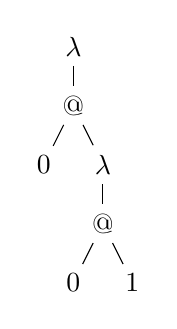
\begin{tikzpicture}[scale=0.5]
	\node{$\lambda$}
	child { node {@}
			child { node {0} }
			child { node {$\lambda$}
					child { node {@} 
						  child {node {0}}
						  child {node {1}}}}} ;
\end{tikzpicture}
\end{figure}

Pour les variables libres, nous pouvons aussi utiliser un indice pour les nommer.
Soit un ensemble de variables libres ${x_1, x_2, x_3,\dots, x_n}$ nous les nommerons en ajoutant 
à leur indice $i$ la profondeur jusqu'à la racine. Les indices des variables libres seront
 donc toujours supérieur à ceux des variables liées sur leurs branches. Cependant, avec cette notation une
 même variable libre avec plusieurs occurences dans un terme pourra avoir des indices différents.

 Nous avons maintenant une représentation \textit{canonique} : deux termes sont $\alpha$-équivalents
 si et seulement si leurs représentations en de de Bruijn sont égales.


Voici une fonction d'implémentation \verb+t2b+ transformant des termes en termes de de Bruijn.
\begin{Verbatim}
let reste s = int_of_string(sub s 1 ((String.length s)-1)) ;;

let add_env var env =
	(var,0)::map (fun pp -> (fst(pp),(1 + snd(pp)))) env ;;

let t2b terme =
	let l = varLibres terme in
	let rec terme_to_bruijn t env hauteur =
	match t with
	| Var x -> if (mem x l) then Va((reste x) + hauteur) else Va(assoc x env)
	| App (n1, n2) -> Ap (terme_to_bruijn n1 env hauteur, terme_to_bruijn n2 env hauteur) 
	| Lam (x, c) -> La (terme_to_bruijn c (add_env x env) (hauteur+1) )
	in terme_to_bruijn terme [] 0

let decalage d t =
	let rec aux p = function
	| Ap (t1,t2) -> Ap (aux p t1, aux p t2) 
	| La (t) -> La (aux (p+1) t)
	| Va (i) when i<p -> Va(i)
	| Va(i) -> Va (i+d)
	in aux 0 t

let beta_b (La u) t =
	let rec aux p = function
	| Ap (u1,u2) -> Ap (aux p u1, aux p u2)
	| La (v) -> La (aux (p+1) v)
	| Va (i)  when i=p -> decalage p t (*on rend t décalé de la profondeur d'abstr p*)
	| Va (i)  when i<p -> Va (i) (*i est lié, on la rend tel quel *)
	| Va (i) -> Va (i-1) (* on décrèmente la variable libre car la betareduc supprime une lamdda*)
	in aux 0 u ;;

let rec normale_bruijn  = function
	| Va x -> raise IRREDUCTIBLE
	| La n -> La (normale_bruijn n)
	| Ap (La n, m) -> beta_b (La n) m
	| Ap (n,m) -> try Ap (normale_bruijn  n, m)
	with IRREDUCTIBLE -> Ap (n, normale_bruijn  m)

let rec reduc_bruijn t =
	try reduc_bruijn (normale_bruijn t)
	with IRREDUCTIBLE -> t 
\end{Verbatim}

Représenter l'ensemble des variables (libres et liées) par un indice de profondeur rend le terme très peu lisible.
La représentation la plus commode semble finalement être d'utiliser la notation de \textit{de Bruijn}  pour les variables liées
 et continuer
à nommer les variables libres par des lettres.

Cela impose dans la définition inductive du terme de distinguer les variables libres des variables liées.

Par exemple en COQ:
\begin{Verbatim}
Inductive terme : Set :=
  | bvar : nat -> terme
  | fvar : string -> terme
  | abs  : terme -> terme
  | app  : terme -> terme -> terme.
\end{Verbatim}